\section{Comparative Analysis}\label{comparativeAnalysis}

Conducting a comparative analysis of 3D models presents a challenging endeavor, as the parameters defining their success vary widely based on the intended application. For instance, low-resolution models suffice for real-time rendering in virtual reality or gaming contexts, whereas the film industry demands high-quality renderings. Similarly, in industrial applications, precision down to the millimeter is crucial, necessitating extremely detailed and accurate meshes. This analysis therefore approaches the assessment of generated models from multiple dimensions:

\begin{enumerate}
    \item \textbf{Prompt/Result Fidelity:} This dimension explores the alignment of each model with the original prompt or image. It questions whether the intended subject of the model is recognizable without prior knowledge of the input, thereby assessing the model's fidelity to the intended design.
    \item \textbf{Geometry:} Here, the focus is on the complexity and intricacy of each model. It evaluates whether the models exhibit detailed, fine structures or lean towards a more generalized, simplistic design. 
    \item \textbf{Texture Realism:} This aspect assesses the authenticity and quality of the textures applied to the models. It delves into questions of realism~-~how real do the textures appear?
\end{enumerate}

Following this subjective analysis, the study proceeds to evaluate technical aspects of each model, focusing on parameters such as rendering time, efficiency, and resource utilization. Each method is also subjected to targeted tests tailored to specific criteria. For instance, in scenarios where symmetry is critical, the models are evaluated for their ability to replicate symmetrical designs. Technical metrics for this analysis are derived from tensorboard data or outputs generated during the model training process. Detailed assessments and quantitative analyses~-~such as the evaluation of symmetry, and the detection of holes or anomalies in the models~-~are examined using Evaluate3D. This custom-developed tool integrates the trimesh Python library \citep{trimesh} to provide insights into the geometric properties of each 3D model.

\subsection{Subjective Evaluation}~\label{subjective}

In the preceding section, it was observed that the methods yielded diverse outcomes when tasked with a broad prompt, such as creating a `robot made of plants'. The text-to-3D methods faced challenges in initially generating an object, a stark contrast to the image-to-3D methods that benefited from having a reference image, offering some directional guidance and hence a slight advantage. To establish a more leveled playing field for the various methods, the next prompt chosen for testing was \textbf{``a high-quality rendering of a Playmobil firefighter''}. Playmobil figures are known for their uniform base structures, differing primarily in clothing or texture. This prompt was therefore selected to assess whether a method could accurately capture the fundamental structure dictated by the prompt. The outcomes of each method, applied to this specific prompt, are illustrated in Figure~\ref{fig:resultPlaymobil}. 

\begin{figure}[ht]
    \centering
    \small
    \begin{subfigure}[b]{0.18\textwidth}
        \centering
        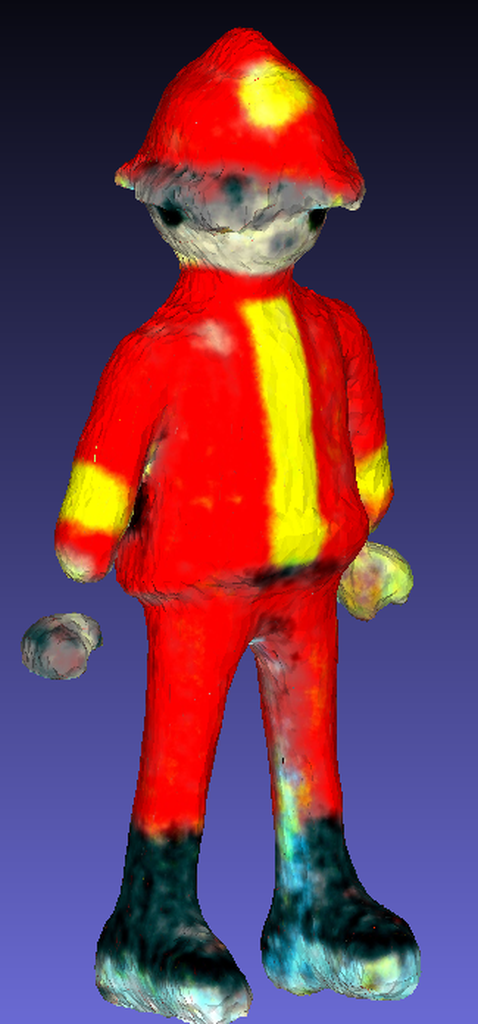
\includegraphics[width=\textwidth]{etc/a high quality rendering of a playmobil firefighter/dreamfusion/dreamfusion_playmobil_result_resize.png}
        \caption{DreamFusion}
    \end{subfigure}
    \begin{subfigure}[b]{0.179\textwidth}
        \centering
        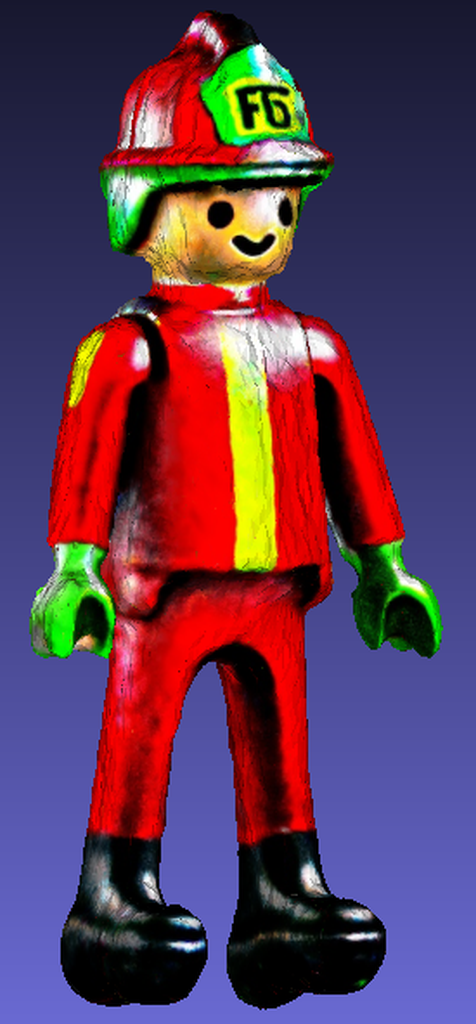
\includegraphics[width=\textwidth]{etc/a high quality rendering of a playmobil firefighter/magic3d/magic3d_playmobil_result_resize.png}
        \caption{Magic3D}
    \end{subfigure}
    \begin{subfigure}[b]{0.227\textwidth}
        \centering
        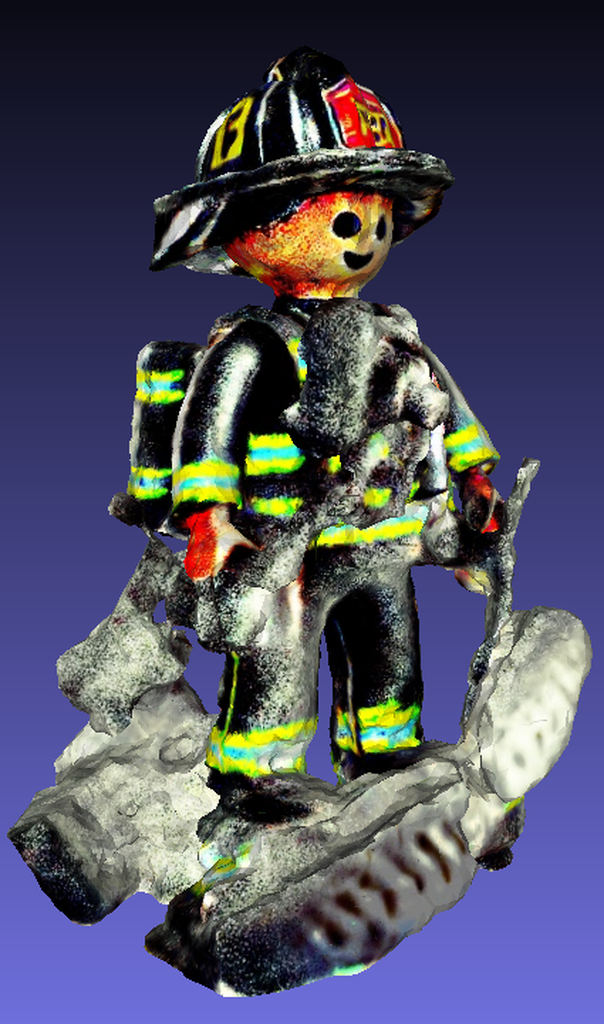
\includegraphics[width=\textwidth]{etc/a high quality rendering of a playmobil firefighter/fantasia3d_Magic3DInput/fantasia_playmobil_result_resize.png}
        \caption{Fantasta3D}
    \end{subfigure}
    \begin{subfigure}[b]{0.192\textwidth}
        \centering
        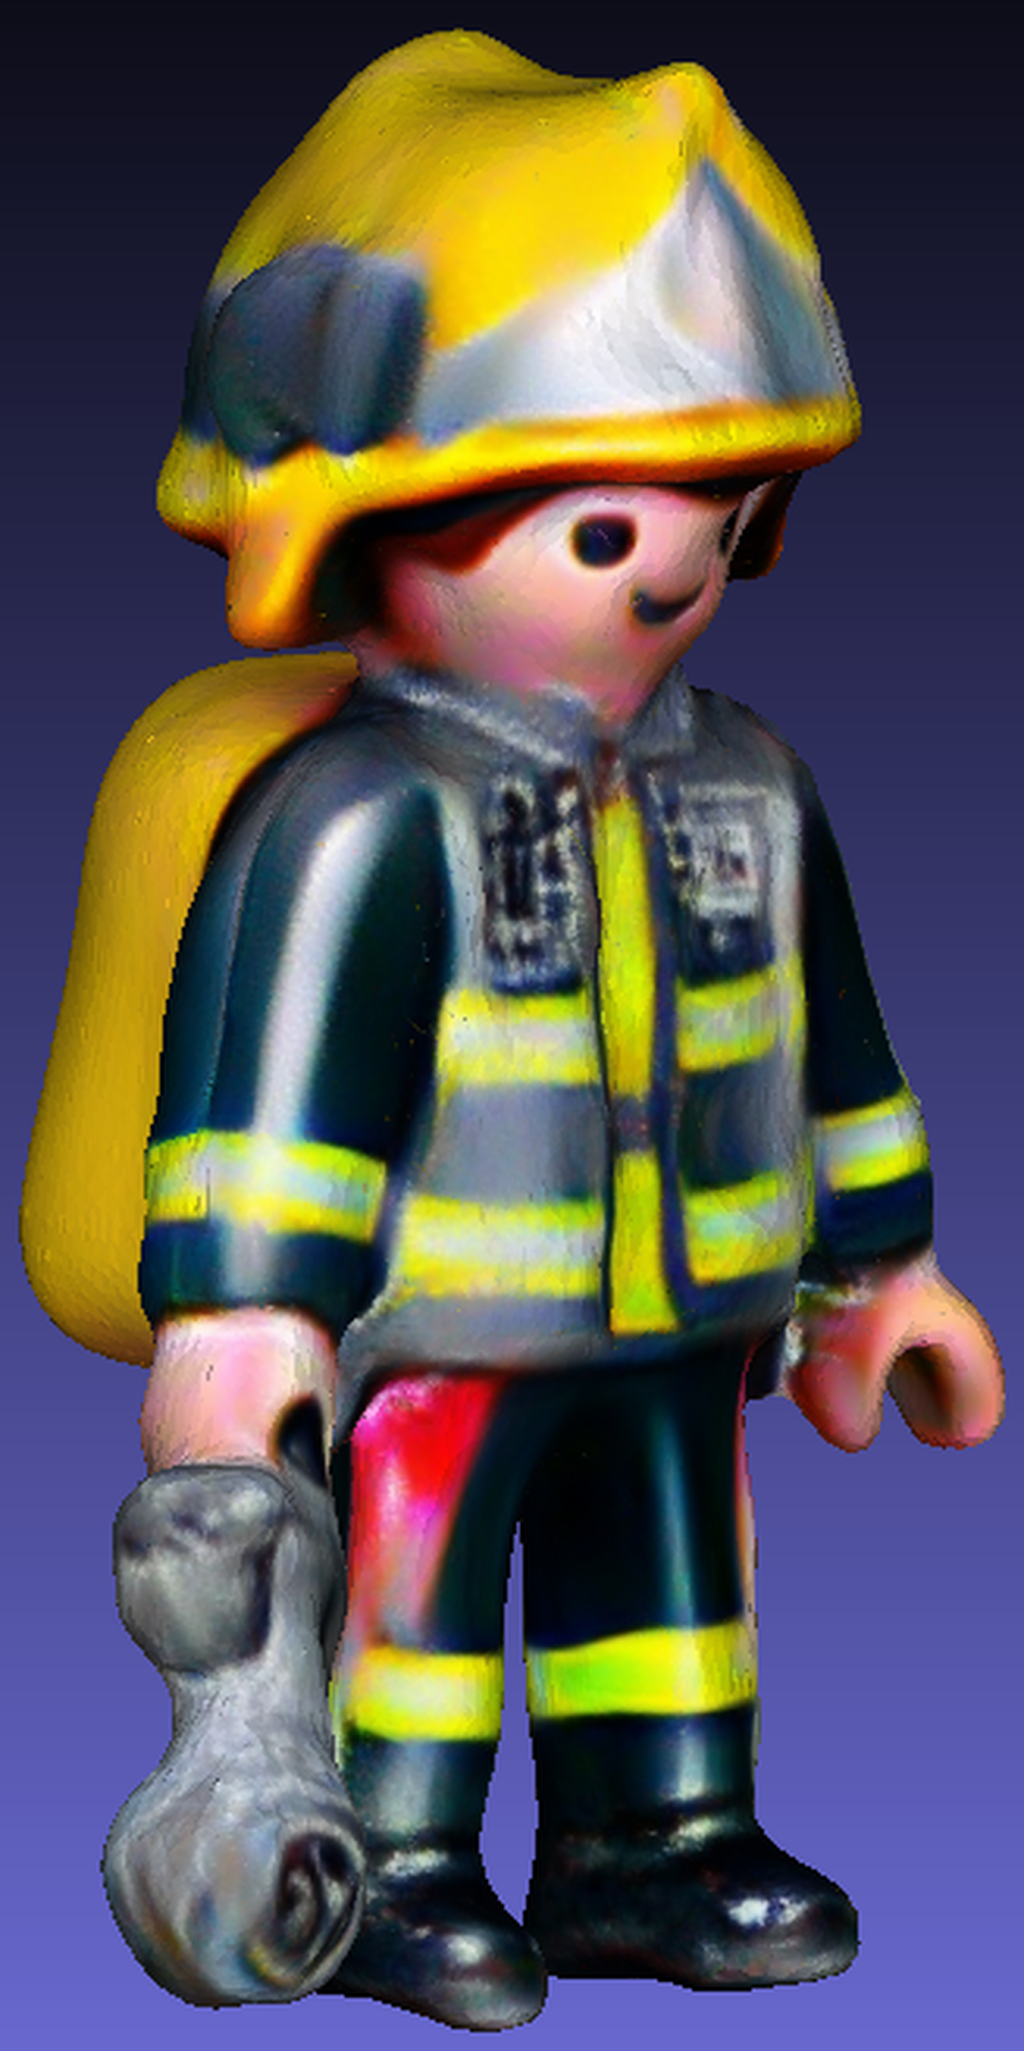
\includegraphics[width=\textwidth]{etc/a high quality rendering of a playmobil firefighter/magic123/magic123_playmobil_result_resize.png}
        \caption{Magic123}
    \end{subfigure}
    \begin{subfigure}[b]{0.181\textwidth}
        \centering
        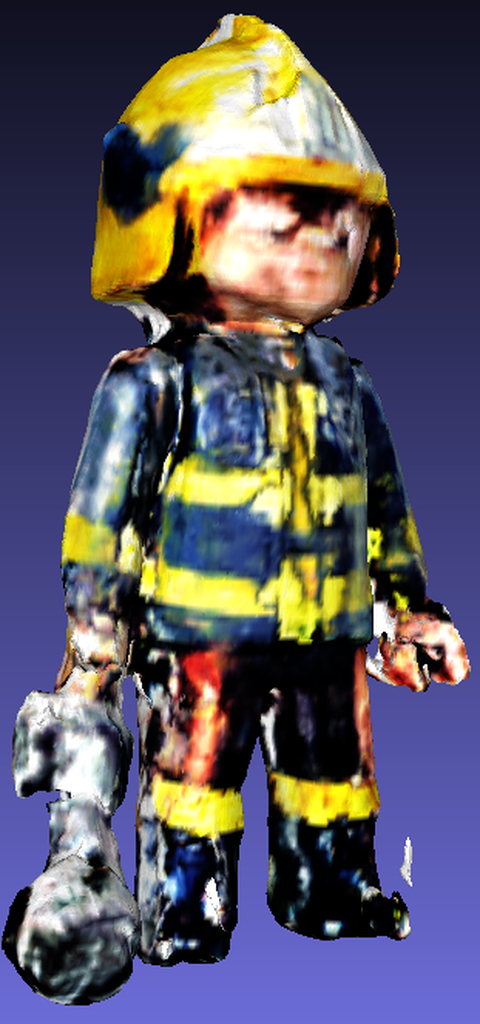
\includegraphics[width=\textwidth]{etc/a high quality rendering of a playmobil firefighter/wonder3D/wonder3d_playmobil_result_resize.png}
        \caption{Wonder3D}
    \end{subfigure}
    \caption{Results obtained using the prompt ``a high-quality rendering of a Playmobil firefighter''.}~\label{fig:resultPlaymobil}
\end{figure}

\textbf{Prompt/Result Fidelity:} There is a clear split in the results when looking at fidelity to the prompt. DreamFusion and Magic123 tend to stick to the red clothing, while Fantasta3D, Magic123 and Wonder3D opt for a more realistic yellow and black firefighter uniform. Wonder3D and Magic123 adapt their results to the expected color scheme of the input image, given in Figure~\ref{fig:inputPlaymobil} part (a). Of particular interest is Fantasta3D's deviation from the red color scheme, although all models were refined with Stable Diffusion. This can be attributed to the physically based material model in the appearance stage, which has learned to associate firefighter clothing with yellow and black rather than red. Each model successfully reproduces identifiable Playmobil features such as helmets and uniforms, although the extent to which they reproduce the Playmobil style varies.

\textbf{Geometry:} The geometric shape of the models varies significantly. DreamFusion and Wonder3D present the most deviations from the expected Playmobil figure geometry. Both exhibit overly smooth shapes with ambiguous edges and floating elements, such as the hands in DreamFusion and around the right foot in Wonder3D, giving an unfinished appearance. In contrast, Fantasta3D achieves a promising silhouette but includes unintended additional objects, like a presumed fire extinguisher on the back and an ambiguous `thing' at the front, possibly an attempt at rendering a fire hose. Magic123, while delivering a solid representation, introduces a large bag on the figure's back, which, unlike the extraneous parts of Fantasta3D, integrates well with the overall model. A closer look of this bag is given in Figure~\ref{fig:inputPlaymobil} parts (b) and (c). Uniquely, Magic123 recreates the iconic Playmobil hand structure, complete with thumb, fingers, and the characteristic gap between them, capturing the essence of the figure's appendages. Magic3D impresses with a near-perfect rendering of the Playmobil figure, capturing the sharp transitions at the joints and maintaining smoothness elsewhere, except for a slight distortion around the feet. This result seems like one could bend and move it like it is possible with an original figure.

\textbf{Texture Realism:} In terms of texture, Magic3D again stands out with a level of realism that surpasses the others for the Playmobil prompt. It boasts clear demarcation between the colors, such as the black of the shoes against the red of the uniform, and the face retains the characteristic Playmobil look. The model's interaction with light, evidenced by chest reflections and inner leg shadows, adds to the plastic appearance. DreamFusion's model lacks such light interplay, resulting in a flat appearance, which is also caused due to the overall smoothened geometry. Fantasta3D, Magic123, and Wonder3D diverge from the red texture, opting for a black and yellow combination with realistic reflective stripes. Fantasta3D's texture is sound despite some geometric artifacts, with light reflection indicating a clear light source and giving the helmet a metallic sheen. Magic123 captures a plastic-like sheen, particularly on the arm's reflection, which underscores the roundness and smoothness of the figure. In contrast, Wonder3D's texture is not very detailed, blurs differences like the separation between jacket and shirt and does not render the character's face, similar to DreamFusion. The whole model looks strange, decayed and unfinished.

\begin{figure}[ht]
    \centering
    \small
    \begin{subfigure}[b]{0.25\textwidth}
        \centering
        
\includegraphics[width=\textwidth]{etc/Images/playmobil.png}
        \caption{}
    \end{subfigure}
    \begin{subfigure}[b]{0.25\textwidth}
        \centering
        
\includegraphics[width=\textwidth]{etc/a high quality rendering of a playmobil firefighter/magic123/magic123_playmobil_refine_back_10000_part1.png}
        \caption{}
    \end{subfigure}
    \begin{subfigure}[b]{0.25\textwidth}
        \centering
        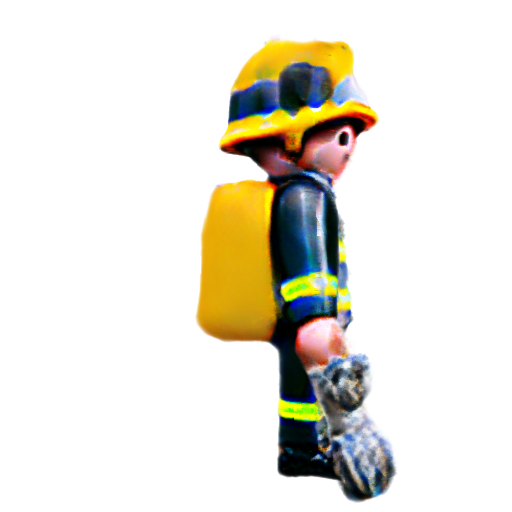
\includegraphics[width=\textwidth]{etc/a high quality rendering of a playmobil firefighter/magic123/magic123_playmobil_coarse_right_10000_part1.png}
        \caption{}
    \end{subfigure}
    \caption{(a) displays the original image for the playmobil figure derived form Dall-E 3; (b and c) show the side and back view of Magic123, resectively}~\label{fig:inputPlaymobil}
\end{figure}

The next prompt used for the various methods was \textbf{``a rendering of a highly symmetrical loaf of bread''}. This prompt was selected to test the precision of each method in replicating detailed, specific requests while still producing coherent results. In this case, the model was tested for its symmetric result capability, which is discussed later in the technical section. The generated models are displayed in Figure~\ref{fig:resultBread}, which includes the original input image created by Dall-E 3 for reference.

Regarding \textbf{Prompt/Result Fidelity}, the outcomes varied. Magic123 and Magic3D successfully captured the essence of a bread, while Wonder3D produced an image that only vaguely suggested a loaf of bread. DreamFusion and Fantasia3D, however, were less successful; the former's result was indistinct, resembling a nondescript lump, while the latter's output more closely resembled a pineapple or an explosion when viewed without context.

\begin{figure}[ht]
    \centering
    \small
    \begin{subfigure}[b]{0.31\textwidth}
        \centering
        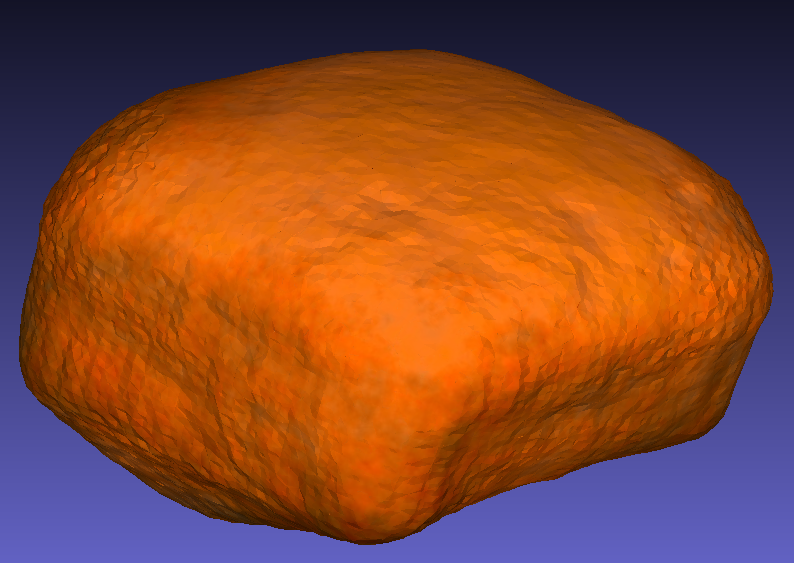
\includegraphics[width=\textwidth]{etc/a rendering of a highly symmetrical loaf of bread/dreamfusion/dreamfusion_bread_result.png}
        \caption{DreamFusion}
        \vspace{0.1cm}
    \end{subfigure}
    \begin{subfigure}[b]{0.31\textwidth}
        \centering
        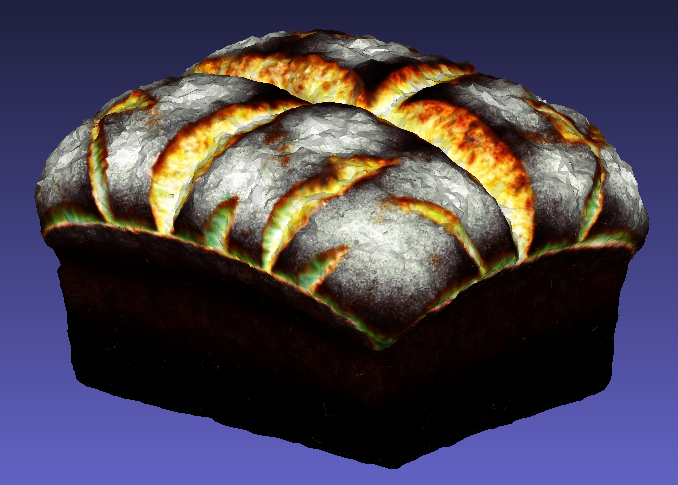
\includegraphics[width=\textwidth]{etc/a rendering of a highly symmetrical loaf of bread/magic3d/magic3D_bread_result.png}
        \caption{Magic3D}
        \vspace{0.1cm}
    \end{subfigure}
    \begin{subfigure}[b]{0.2\textwidth}
        \centering
        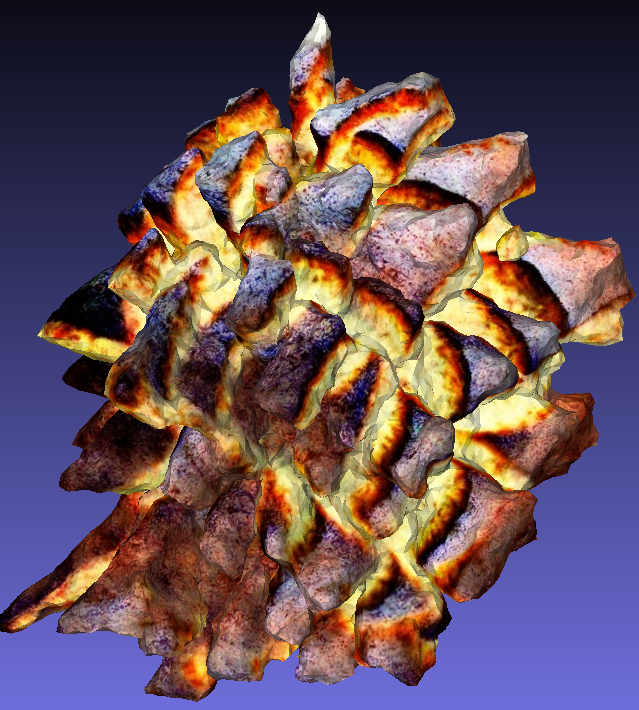
\includegraphics[width=\textwidth]{etc/a rendering of a highly symmetrical loaf of bread/fantasia3d/fantasia_bread_result.png}
        \caption{Fantasta3D}
        \vspace{0.1cm}
    \end{subfigure}

    \begin{subfigure}[b]{0.269\textwidth}
        \centering
        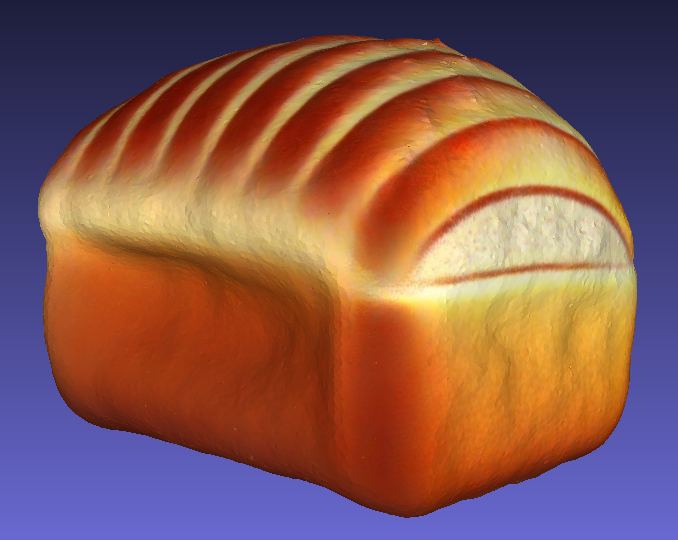
\includegraphics[width=\textwidth]{etc/a rendering of a highly symmetrical loaf of bread/magic123/magic123_bread_result.png}
        \caption{Magic123}
        \vspace{0.1cm}
    \end{subfigure}
    \begin{subfigure}[b]{0.23\textwidth}
        \centering
        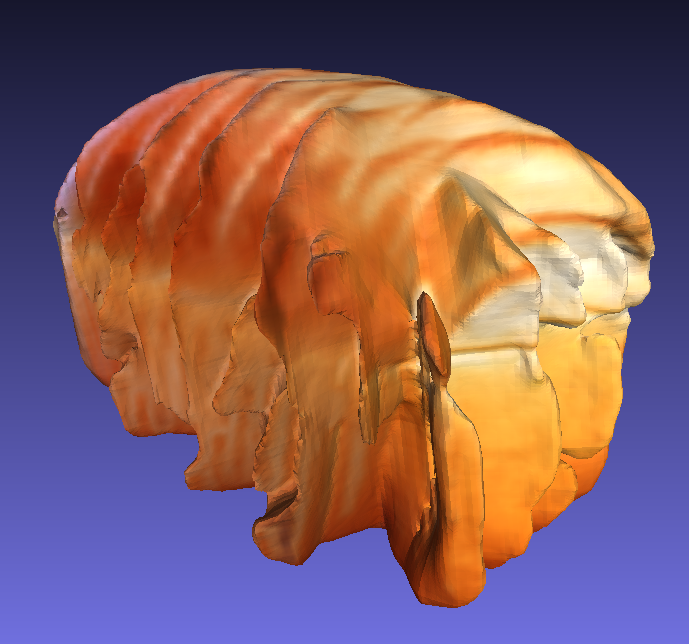
\includegraphics[width=\textwidth]{etc/a rendering of a highly symmetrical loaf of bread/wonder3D/wonder3d_bread_result.png}
        \caption{Wonder3D}
        \vspace{0.1cm}
    \end{subfigure}
    \begin{subfigure}[b]{0.23\textwidth}
        \centering
        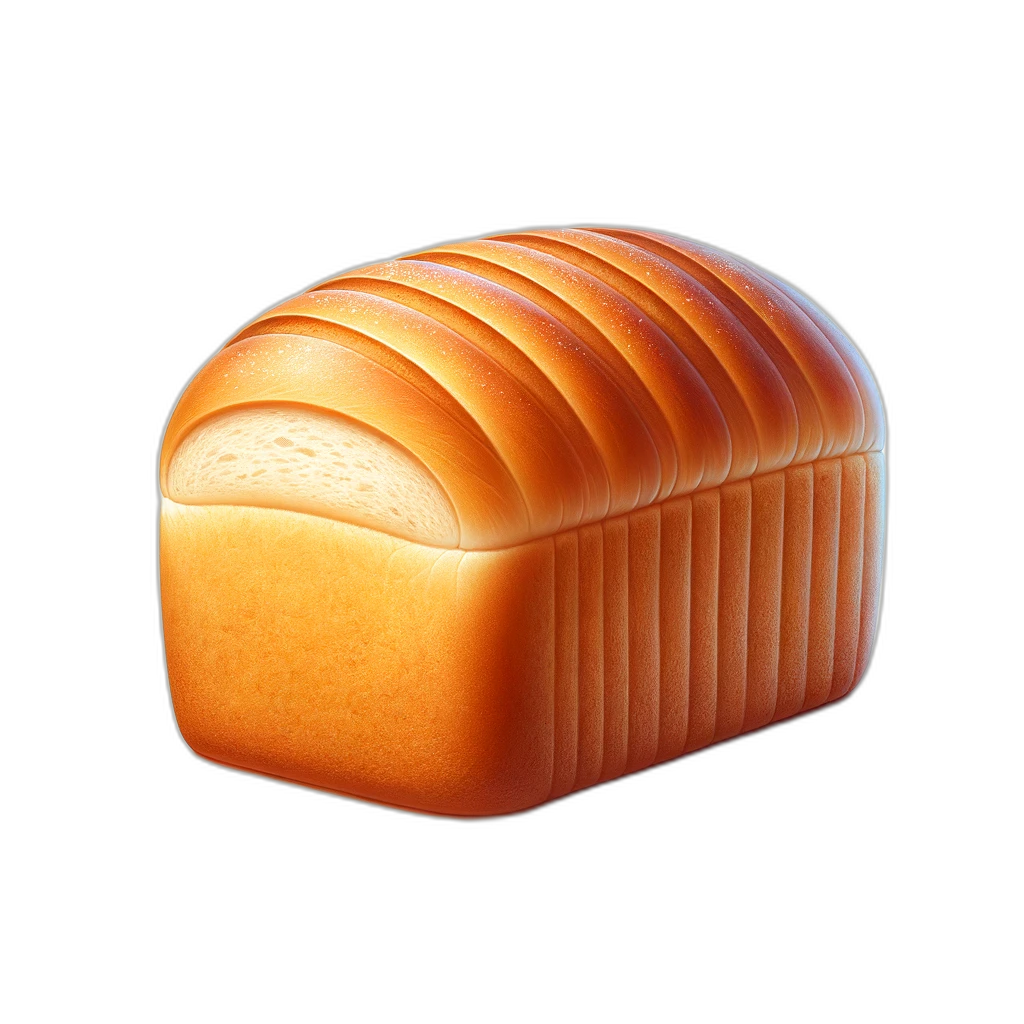
\includegraphics[width=\textwidth]{etc/Images/bread.png}
        \caption{Original Image}
        \vspace{0.1cm}
    \end{subfigure}
    \caption{Results obtained using the prompt ``a rendering of a highly symmetrical loaf of bread''. Part (f) is the input image for Magic123 and Wonder3D, generated with Dall-E 3}~\label{fig:resultBread}
\end{figure}

In terms of \textbf{Geometry}, DreamFusion's model lacked meaningful structure, while Magic3D's bread model achieved good geometry, with a realistically carved top resembling fresh black bread. Fantasia3D, on the other hand, produced a model with a spikey appearance, potentially due to overfitting or difficulty in determining a starting point for the flat bottom of the bread. Magic123 excelled in replicating the geometry of the input image, closely matching the cuts and overall shape of the bread. Conversely, Wonder3D's model, like Fantasia3D's, had a roughly bread-like shape but suffered from spikey edges, possibly due to small adjustments during 3D mesh generation.

When considering \textbf{Texture Realism}, only the textures from Magic3D, Fantasia3D, and Magic123 seemed noteworthy. Magic3D's texture gave the impression of a burnt, dark loaf, with a realistic color gradient on the top. Although Fantasia3D's texture had a pleasing color combination, it resembled a cluster of breadsticks unless contextual information was provided. Magic123 accurately replicated the texture of the original image, demonstrating its proficiency in handling low-detail requirements.

To assess the methods' capability in reproducing smooth and reflective textures along with complex environmental details, the prompt \textbf{``a highly polished, seamless chrome sphere reflecting a complex cityscape in bright daylight''} was employed.





For a comprehensive evaluation of the methods' ability to render lifelike organic forms and textures, the prompt \textbf{``a high-quality rendering of a big dog sleeping on a chair''} was used. This particular prompt aims to test the realism in fur texture and the anatomical precision of the rendered dog.





To further explore each method's proficiency in rendering detailed natural elements and contrasting materials, the prompt \textbf{``a high-quality rendering of a fern in a wooden pot''} was introduced. This prompt serves to assess the handling of complex details in natural subjects, as well as the accuracy of color gradients and lighting in various levels of depth.


\begin{figure}[ht]
    \centering
    \small
    \begin{subfigure}[b]{0.24\textwidth}
        \centering
        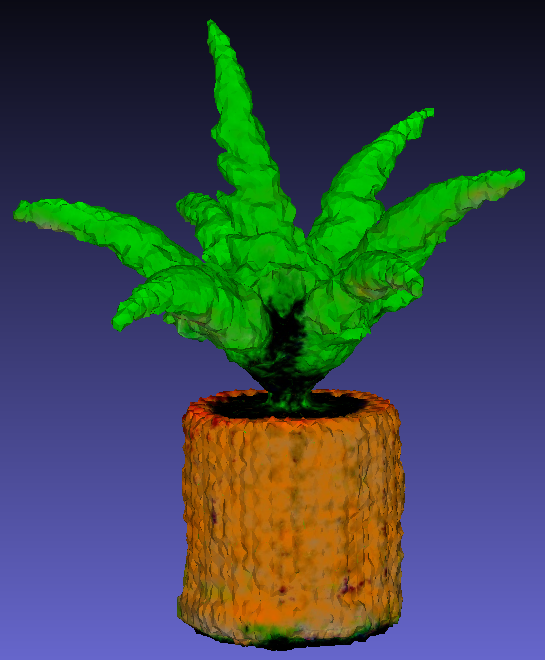
\includegraphics[width=\textwidth]{etc/a high-quality rendering of a fern in a wooden pot/dreamfusion/dreamfusion_fern_result.png}
        \caption{DreamFusion}
        \vspace{0.1cm}
    \end{subfigure}
    \begin{subfigure}[b]{0.35\textwidth}
        \centering
        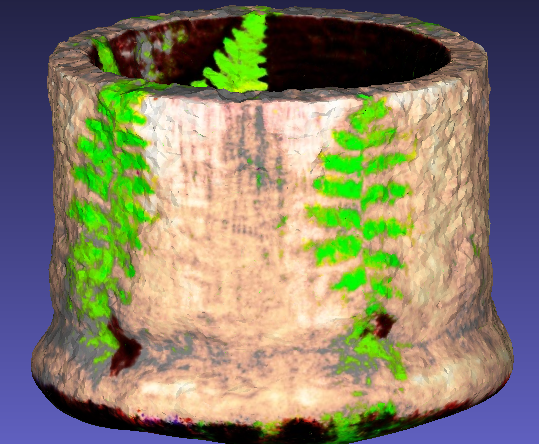
\includegraphics[width=\textwidth]{etc/a high-quality rendering of a fern in a wooden pot/magic3d/magic3d_fern_result.png}
        \caption{Magic3D}
        \vspace{0.1cm}
    \end{subfigure}
    \begin{subfigure}[b]{0.32\textwidth}
        \centering
        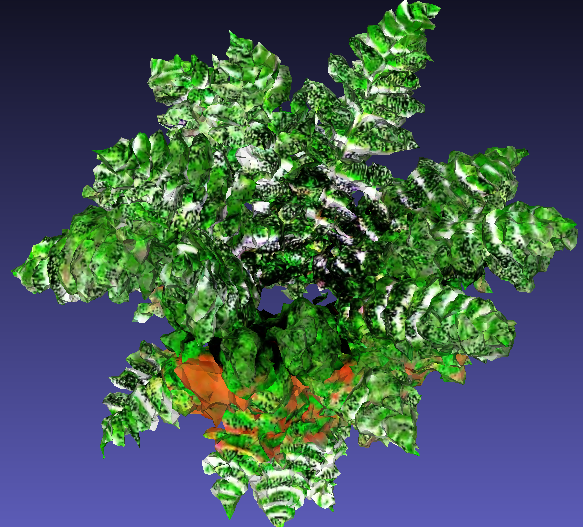
\includegraphics[width=\textwidth]{etc/a high-quality rendering of a fern in a wooden pot/fantasia3d/fantasia_fern_result.png}
        \caption{Fantasta3D}
        \vspace{0.1cm}
    \end{subfigure}

    \begin{subfigure}[b]{0.28\textwidth}
        \centering
        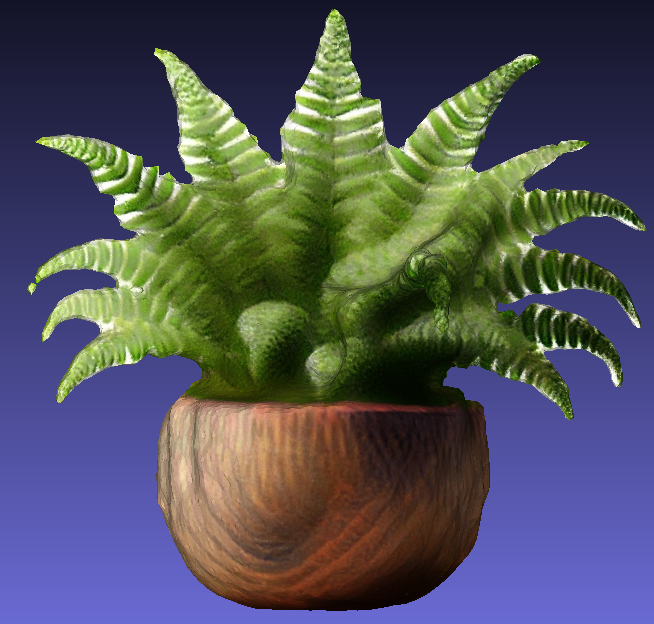
\includegraphics[width=\textwidth]{etc/a high-quality rendering of a fern in a wooden pot/magic123/magic123_fern_front_result.png}
        \caption{Magic123}
        \vspace{0.1cm}
    \end{subfigure}
    \begin{subfigure}[b]{0.27\textwidth}
        \centering
        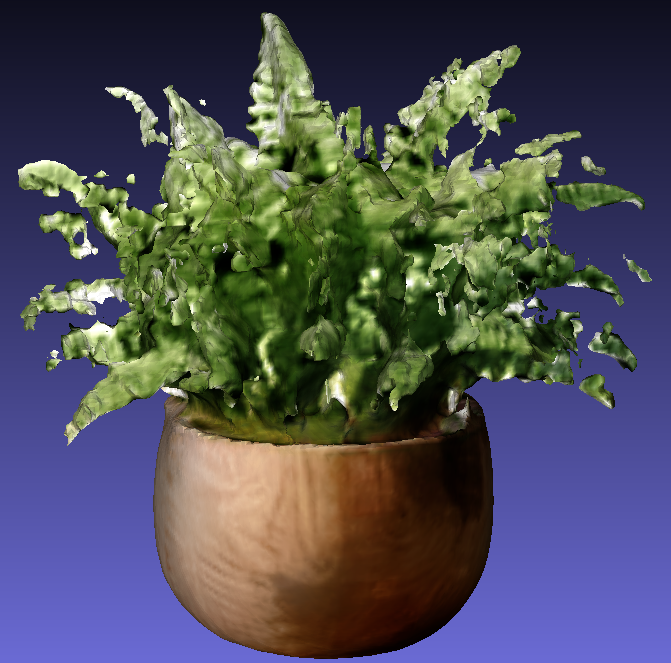
\includegraphics[width=\textwidth]{etc/a high-quality rendering of a fern in a wooden pot/wonder3D/wonder3d_fern_result.png}
        \caption{Wonder3D}
        \vspace{0.1cm}
    \end{subfigure}
    \begin{subfigure}[b]{0.28\textwidth}
        \centering
        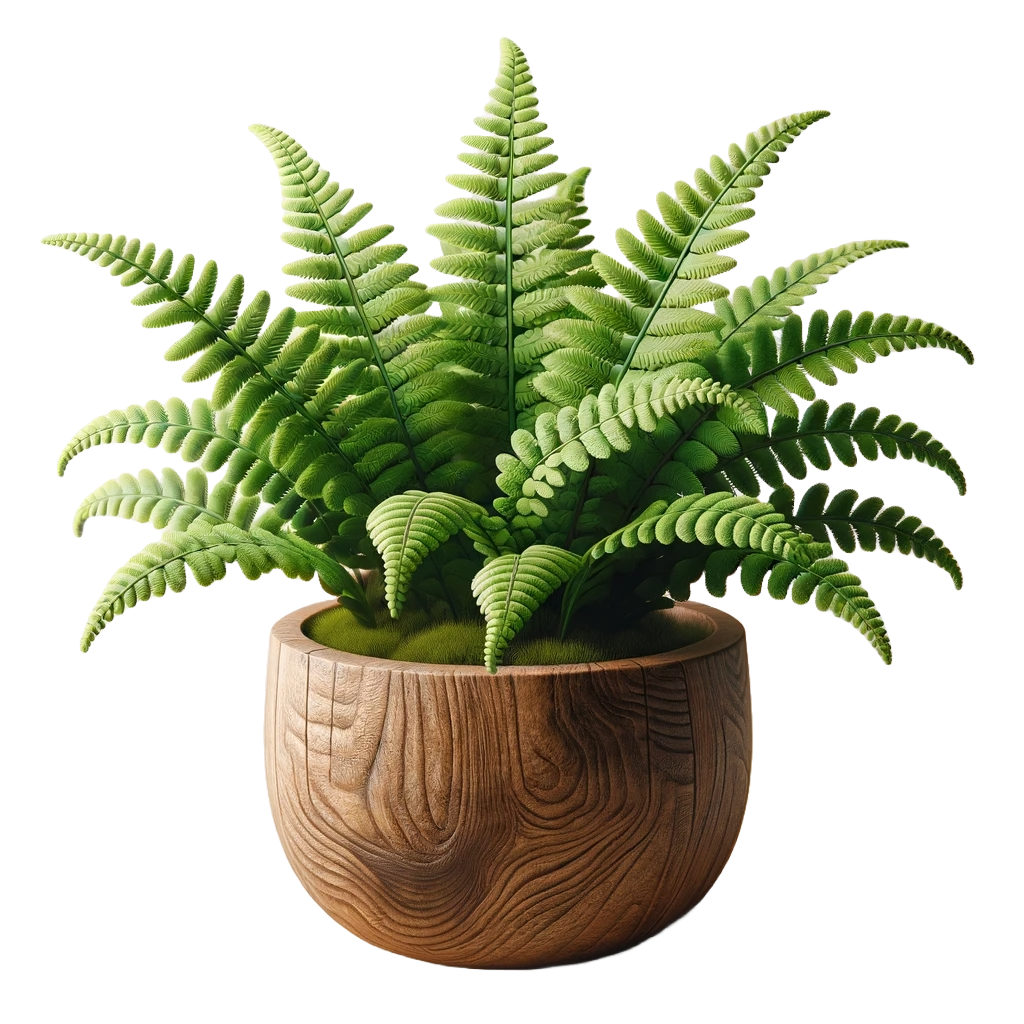
\includegraphics[width=\textwidth]{etc/Images/fern.png}
        \caption{Original Image}
        \vspace{0.1cm}
    \end{subfigure}
    \caption{Results obtained using the prompt ``a high-quality rendering of a fern in a wooden pot''.}~\label{fig:resultFern}
\end{figure}


\begin{figure}[ht]
    \centering
    \begin{subfigure}[b]{0.2\textwidth}
        \centering
        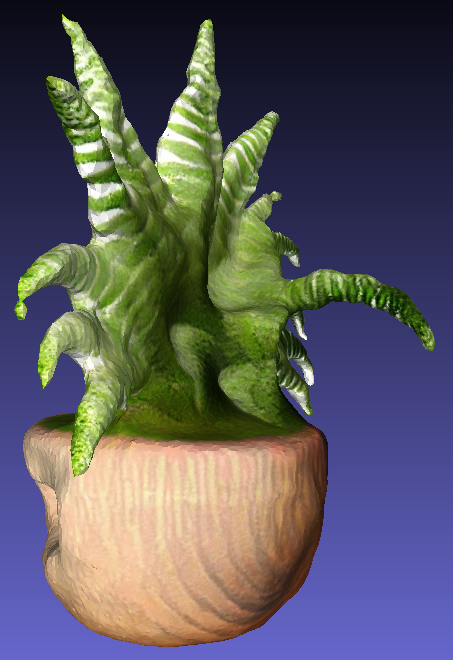
\includegraphics[width=\textwidth]{etc/a high-quality rendering of a fern in a wooden pot/magic123/magic123_fern_side_result.png}
        \caption{Magic123}
    \end{subfigure}
    \begin{subfigure}[b]{0.32\textwidth}
        \centering
        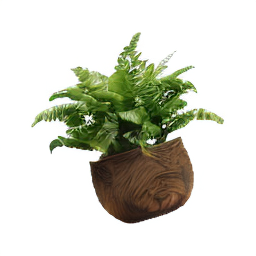
\includegraphics[width=\textwidth]{etc/a high-quality rendering of a fern in a wooden pot/wonder3D/rgb_000_right.png}
        \caption{Wonder3D}
    \end{subfigure}
    \caption{The side view of the fern showcasing the limitations of Magic123 in deriving the correct angles}\label{fig:fernSideview}
  \end{figure}



  \begin{figure}[ht]
    \centering
    \small
    \begin{subfigure}[b]{0.295\textwidth}
        \centering
        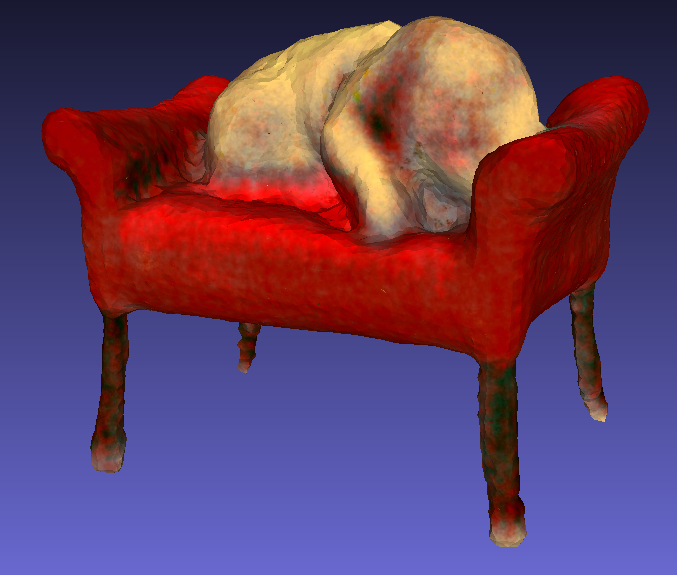
\includegraphics[width=\textwidth]{etc/a high-quality rendering of a big dog sleeping on a chair/dreamfusion/dreamfusion_dog_front_result.png}
        \caption{DreamFusion}
        \vspace{0.1cm}
    \end{subfigure}
    \begin{subfigure}[b]{0.32\textwidth}
        \centering
        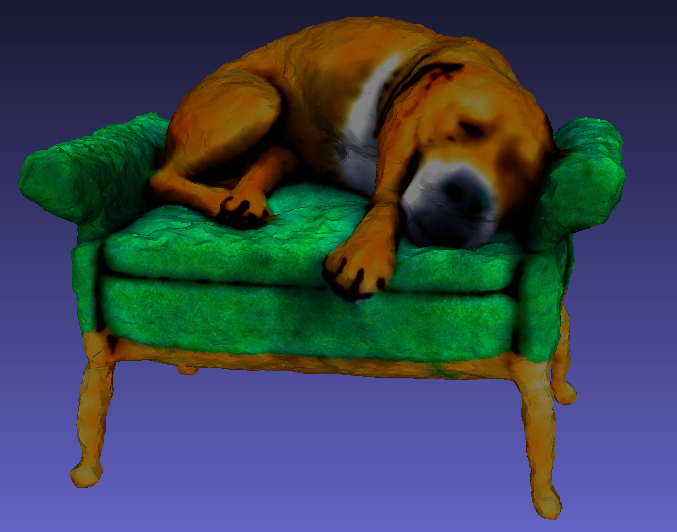
\includegraphics[width=\textwidth]{etc/a high-quality rendering of a big dog sleeping on a chair/magic3d/magic3D_dog_front_result.png}
        \caption{Magic3D}
        \vspace{0.1cm}
    \end{subfigure}
    \begin{subfigure}[b]{0.33\textwidth}
        \centering
        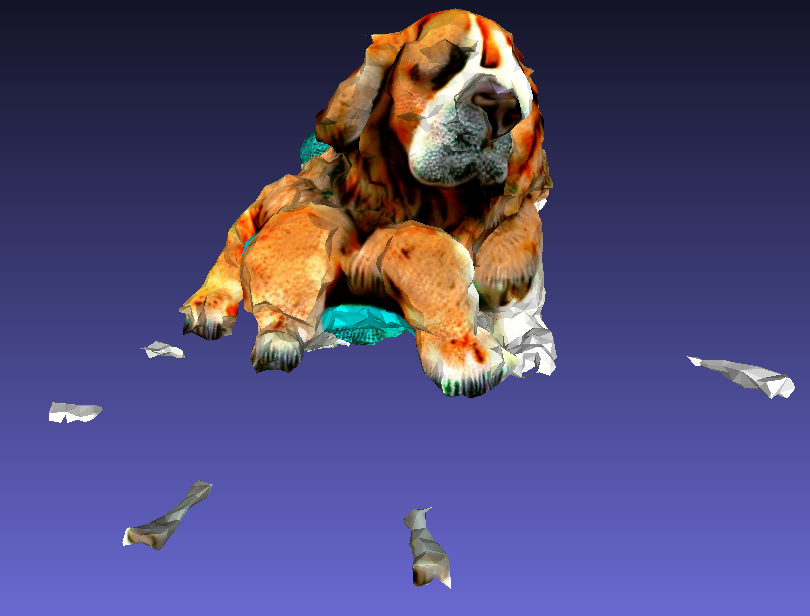
\includegraphics[width=\textwidth]{etc/a high-quality rendering of a big dog sleeping on a chair/fantasia3d/fantasia_dog_front_result.png}
        \caption{Fantasta3D}
        \vspace{0.1cm}
    \end{subfigure}

    \begin{subfigure}[b]{0.267\textwidth}
        \centering
        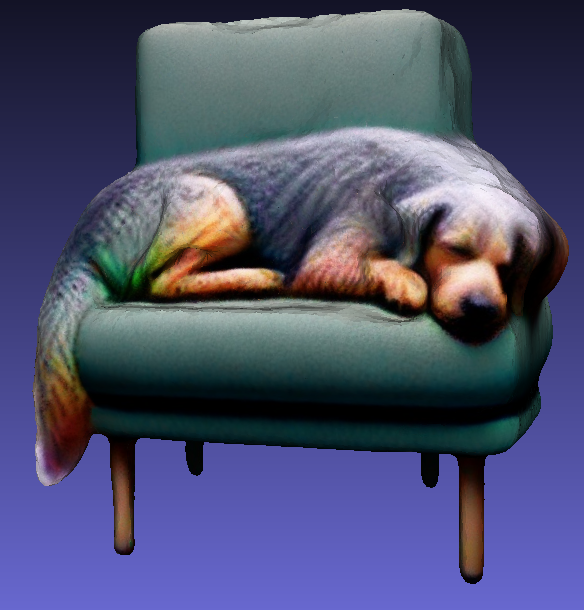
\includegraphics[width=\textwidth]{etc/a high-quality rendering of a big dog sleeping on a chair/magic123/magic123_dog_front_result.png}
        \caption{Magic123}
        \vspace{0.1cm}
    \end{subfigure}
    \begin{subfigure}[b]{0.27\textwidth}
        \centering
        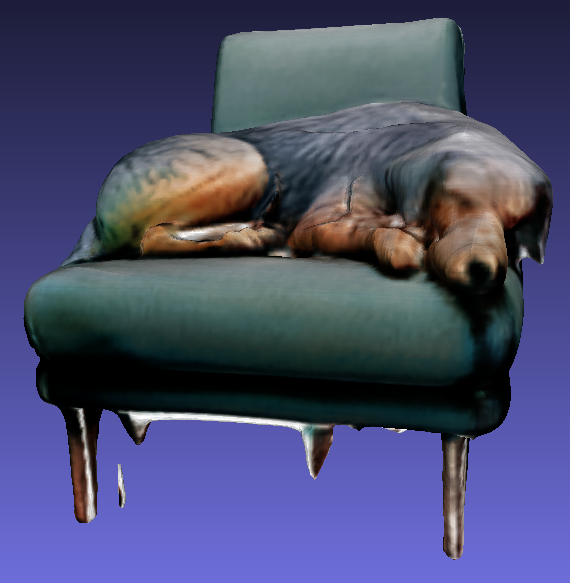
\includegraphics[width=\textwidth]{etc/a high-quality rendering of a big dog sleeping on a chair/wonder3D/wonder3D_dog_front_result.png}
        \caption{Wonder3D}
        \vspace{0.1cm}
    \end{subfigure}
    \begin{subfigure}[b]{0.28\textwidth}
        \centering
        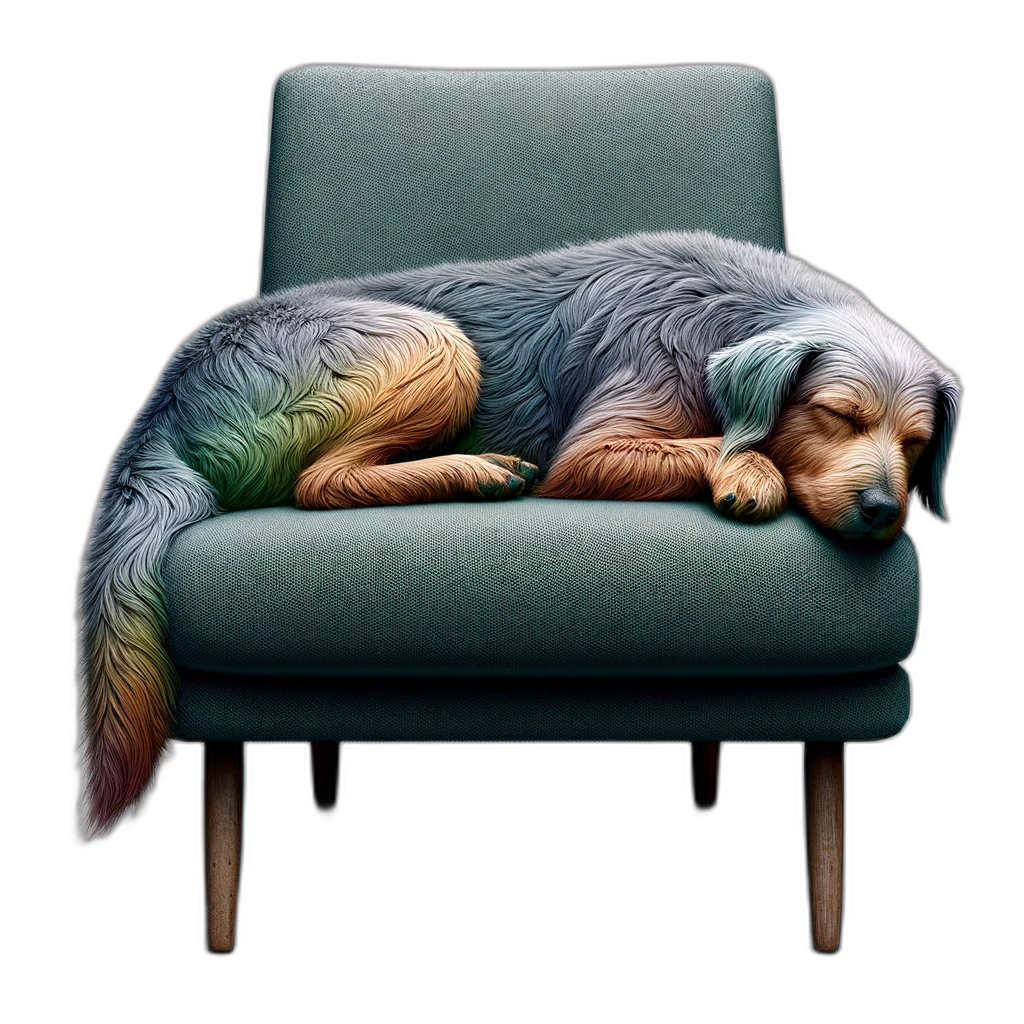
\includegraphics[width=\textwidth]{etc/Images/dog.png}
        \caption{Original Image}
        \vspace{0.1cm}
    \end{subfigure}
    \caption{Results obtained using the prompt ``a high-quality rendering of a big dog sleeping on a chair''.}~\label{fig:resultDogFront}
\end{figure}


\begin{figure}[ht]
    \centering
    \small
    \begin{subfigure}[b]{0.291\textwidth}
        \centering
        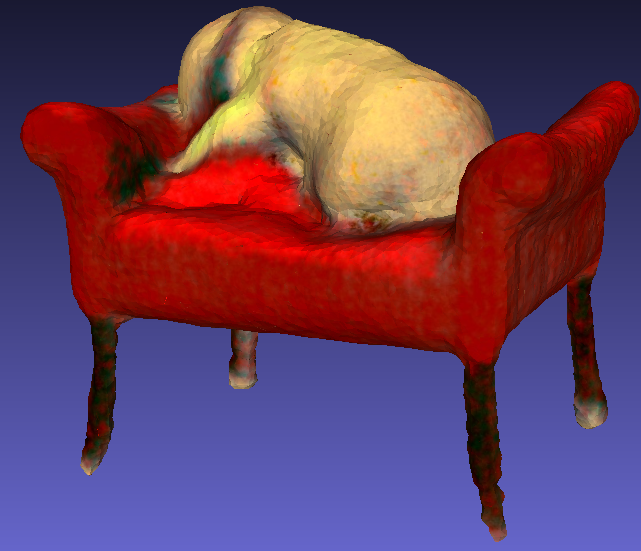
\includegraphics[width=\textwidth]{etc/a high-quality rendering of a big dog sleeping on a chair/dreamfusion/dreamfusion_dog_back_result.png}
        \caption{DreamFusion}
        \vspace{0.1cm}
    \end{subfigure}
    \begin{subfigure}[b]{0.3\textwidth}
        \centering
        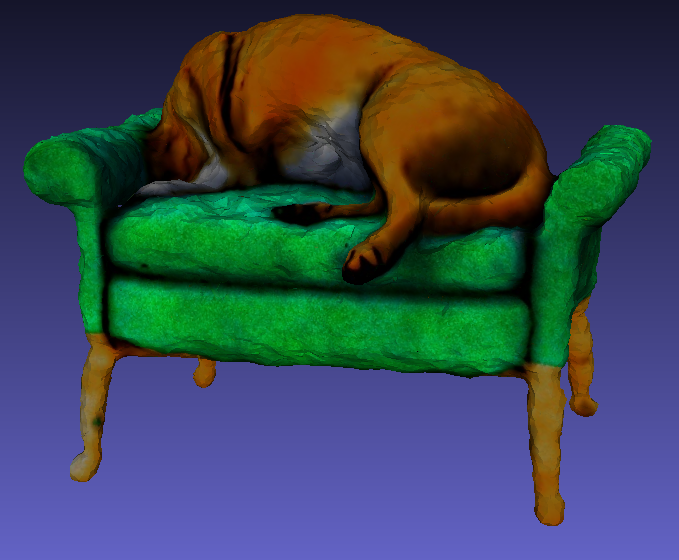
\includegraphics[width=\textwidth]{etc/a high-quality rendering of a big dog sleeping on a chair/magic3d/magic3D_dog_back_result.png}
        \caption{Magic3D}
        \vspace{0.1cm}
    \end{subfigure}
    \begin{subfigure}[b]{0.34\textwidth}
        \centering
        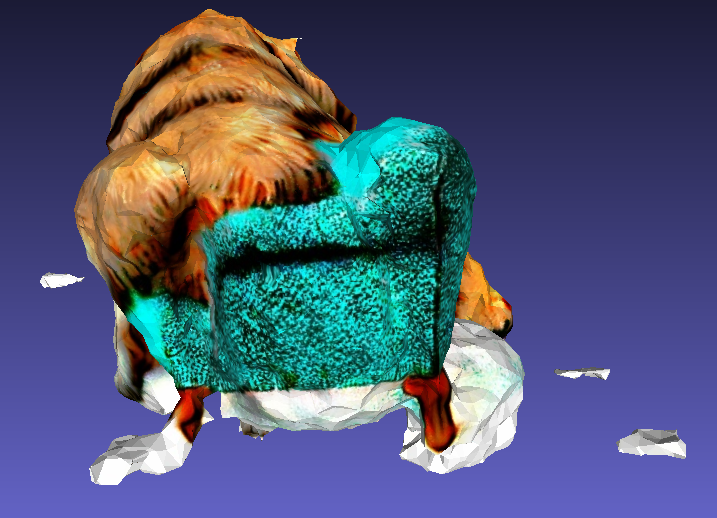
\includegraphics[width=\textwidth]{etc/a high-quality rendering of a big dog sleeping on a chair/fantasia3d/fantasia_dog_back_result.png}
        \caption{Fantasta3D}
        \vspace{0.1cm}
    \end{subfigure}

    \begin{subfigure}[b]{0.261\textwidth}
        \centering
        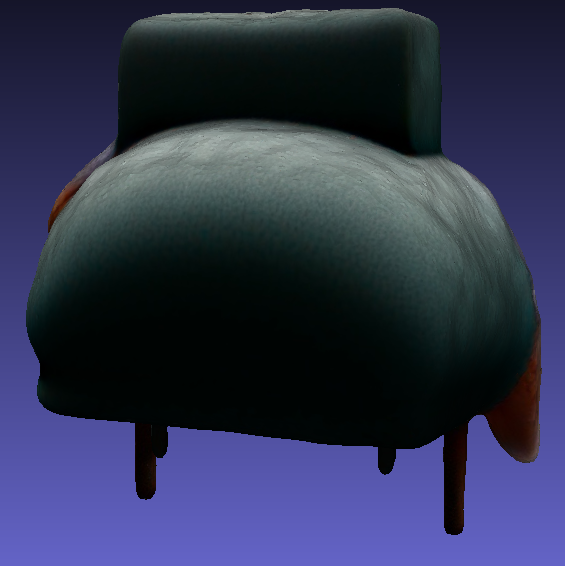
\includegraphics[width=\textwidth]{etc/a high-quality rendering of a big dog sleeping on a chair/magic123/magic123_dog_back_result.png}
        \caption{Magic123}
        \vspace{0.1cm}
    \end{subfigure}
    \begin{subfigure}[b]{0.27\textwidth}
        \centering
        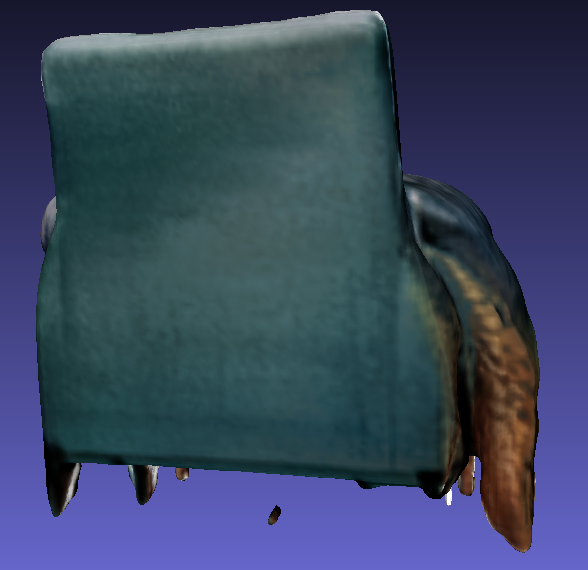
\includegraphics[width=\textwidth]{etc/a high-quality rendering of a big dog sleeping on a chair/wonder3D/wonder3D_dog_back_result.png}
        \caption{Wonder3D}
        \vspace{0.1cm}
    \end{subfigure}
    \caption{Results obtained using the prompt ``a high-quality rendering of a big dog sleeping on a chair''.}~\label{fig:resultDogBack}
\end{figure}
\subsection{Technical Review}~\label{technical}

playmobil

The effectiveness of Evaluate3D is further enhanced by the integration of OpenAI's CLIP-score, a metric that quantifies the correspondence between an image and a given prompt \citep{radfordCLIP}. This is achieved by encoding both the prompt and the image into high-dimensional vectors within the same embedding space, and then determining the cosine similarity between these vectors. Cosine similarity is a measure of orientation rather than magnitude, with the cosine of the angle between two vectors indicating how closely the content of the image mirrors that of the text prompt. Despite its sophisticated design, this score is not without limitations and at times cannot rival the discerning capabilities of the human eye, occasionally leading to outcomes that may seem counterintuitive.

For convenience and to streamline the evaluation process, portions of the code using this metric have been integrated into Evaluate3D. This enables an immediate calculation of the CLIP-score post-rendering. Utilizing this feature, scores for the Playmobil figures have been computed and are presented in Table~\ref{table:scorePlaymobil}. In an intriguing turn, Magic123 ranks highest when assessed against the original prompt, followed by Fantasia3D, Wonder3D, DreamFusion, and finally, Magic3D. These findings are not entirely in concordance with the subjective analysis provided earlier. However, when the prompt is changed to ``a high-quality rendering of a red Playmobil firefighter'', there is a marked reversal in scores. This suggests that the CLIP-score may exhibit a bias towards the color black in the context of firefighter apparel, as opposed to the more toy-like red. The discrepancies highlighted by the CLIP-score accentuate the need for the development of new, more precise evaluation metrics tailored for assessing the output of 3D generative AI, as there currently exists no standard method that is universally recognized as reliable.

\begin{table}[h]
    \centering
    \small
    \begin{tabular}{lccccc}
    \toprule
    Prompt & DreamFusion & Magic3D & Fantasia3D & Magic123 & Wonder3D \\
    \midrule
    a Playmobil firefighter & 0.337 & 0.320 & 0.503 & 0.827 & 0.482 \\
    a red Playmobil firefighter & 0.501 & 0.604 & 0 & 0 & 0.216 \\
    \bottomrule
    \end{tabular}
    \caption{CLIP-scores for Playmobil firefighter models based on different prompts.}~\label{table:scorePlaymobil}
\end{table}


Bread

To quantitatively assess the symmetry of each model, the study employed Evaluate3D. This tool uses a function from trimesh to mirror a model along an axis and checks for corresponding vertices on the mirrored side. This process is repeated for all vertices, and a symmetry score is derived based on the number of matching pairs found. The findings of this assessment are detailed in Table~\ref{table:symmetrieBread}.

\begin{table}[ht]
    \centering
    \small
    \begin{tabular}{lccccc}
    \toprule
    {} & DreamFusion & Magic3D & Fantasia3D & Magic123 & Wonder3D \\
    \midrule
    Symmetrie Score & 0.337 & 0.320 & 0.503 & 0.827 & 0.482 \\
    \bottomrule
    \end{tabular}
    \caption{Symmetrie-scores for bread models demanding a symmetrical output.}~\label{table:symmetrieBread}
\end{table}



The blow table shows the rendering times required for each prmompt with each model. 

\begin{table}[ht]
    \centering
    \small 
    \begin{tabular}{lcccccccc}
    \toprule
    Prompt & DreamFusion & \multicolumn{2}{c}{Magic3D} & \multicolumn{2}{c}{Fantasia3D} & \multicolumn{2}{c}{Magic123} & Wonder3D \\
    \cmidrule(r){3-4} \cmidrule(lr){5-6} \cmidrule(l){7-8}
    & & \multicolumn{1}{c}{Coarse} & \multicolumn{1}{c}{Refine} & \multicolumn{1}{c}{Geom.} & \multicolumn{1}{c}{Appear.} & \multicolumn{1}{c}{C.} & \multicolumn{1}{c}{R.} &  \\
    \midrule
    Robot & 1:24 & 1:23 & 1:20 & 1:15 & 1:18 & 1:46 & 1:47 & 0:15 \\
    Playmobil & 1:17 & 1:17 & 1:18 & 1:14 & 1:17 & 1:46 & 1:46 & 0:15 \\
    Fern & 1:25 & 1:24 & 1:19 & 1:17 & 1:20 & 1:52 & 1:48 & 0:15 \\
    Bread & 1:25 & 1:21 & 1:21 & 1:17 & 1:20 & 1:54 & 1:52 & 0:15 \\
    \bottomrule
    \end{tabular}
    \caption{Comparison of Generation Times for Different Prompts Across Methods (Hours:Minutes). Legend: C = Coarse, R = Refine, Geom = Geometry, Appear = Appearance.}~\label{table:generation_times_complex}
\end{table}

 
    
    
    